\documentclass[10pt]{beamer}

\usetheme[progressbar=frametitle]{metropolis}
\usepackage{appendixnumberbeamer}
\definecolor{maincolor}{RGB}{35, 55, 58}
\usepackage{booktabs}
\usepackage[scale=2]{ccicons}
\usepackage{tcolorbox}
\tcbuselibrary{theorems}
\usepackage{pgfplots}
\usepgfplotslibrary{dateplot}
\usepackage{xspace}
\usepackage{tikz-cd}
\setbeamercovered{transparent}
\newcommand{\themename}{\textbf{\textsc{metropolis}}\xspace}
\usepackage{graphicx}
\usepackage{subcaption}
\graphicspath{ {./images/} }




% {{{
\def\sh{\mathcal}                   % sheaf font
\def\bb{\mathbb}                    % bold font
\def\cat{\mathtt}                   % category font
\def\leq{\leqslant}                 % <=
\def\geq{\geqslant}                 % >=
\def\setmin{-}                      % set minus
\def\rad{\mathfrak{r}}              % radical
\def\nilrad{\mathfrak{N}}           % nilradical
\def\emp{\varnothing}               % empty set
\def\vphi{\phi}                     % for switching \phi and \varphi, change if needed
\def\HH{\mathrm{H}}                 % cohomology H
\def\CHH{\check{\HH}}               % Čech cohomology H
\def\RR{\mathrm{R}}                 % right derived R
\def\LL{\mathrm{L}}                 % left derived L
\def\dual#1{{#1}^\v}              % dual
\def\v{\smash{\scalebox{.8}[1.4]{\rotatebox{90}{\guilsinglleft}}}}
\def\kres{k}                        % residue field k
\def\C{\cat{C}}                     % category C
\def\op{^\cat{op}}                  % opposite category
\def\Set{\cat{Set}}                 % category of sets
\def\CHom{\cat{Hom}}                % functor category
\def\supertilde{{\,\widetilde{\,}\,}}   % use \supertilde instead of ^\sim
\def\GL{\bb{GL}}
\def\Q{\bb{Q}}
\def\Z{\bb{Z}}
\def\R{\bb{R}}
\def\C{\bb{C}}
\def\O{\sh{O}}
\def\G{\bb{G}}
\def\P{\bb{P}}
\def\bbGamma{\boldsymbol\Gamma}
\def\red{\mathrm{red}}
\def\rg{\operatorname{rg}}
\def\gr{\operatorname{gr}}
\def\Gr{\operatorname{Gr}}
\def\Sym{\operatorname{Sym}}
\def\Hom{\operatorname{Hom}}
\def\Proj{\operatorname{Proj}}
\def\Tor{\operatorname{Tor}}
\def\Ext{\operatorname{Ext}}
\def\Supp{\operatorname{Supp}}
\def\Ker{\operatorname{Ker}}
\def\Im{\operatorname{Im}}
\def\Coker{\operatorname{Coker}}
\def\Spec{\operatorname{Spec}}
\def\Spf{\operatorname{Spf}}
\def\grad{\operatorname{grad}}
\def\dimc{\operatorname{dimc}}
\def\codim{\operatorname{codim}}
\def\id{\operatorname{id}}
\def\Der{\operatorname{Der}}
\def\Diff{\operatorname{Diff}}
\def\Hyp{\operatorname{Hyp}}
\def\Tr{\operatorname{Tr}}
% }}}

\newtcbtheorem{colordef}{Definition} {theorem style = plain, colback=maincolor!30!white, coltitle=black, colframe=black, fonttitle = \upshape\bfseries, fontupper=\itshape}{th}

\newtcbtheorem[no counter]{colorthm}{Theorem} {theorem style = plain, colback=maincolor!30!white, coltitle=black, colframe=white, fonttitle = \upshape\bfseries, fontupper=\itshape}{th}

\newtcbtheorem[no counter]{colorconj}{Conjecture} {theorem style = plain, colback=maincolor!30!white, coltitle=black, colframe=white, fonttitle = \upshape\bfseries, fontupper=\itshape}{conj}

\newtcbtheorem{constructionbox}{Construction} {theorem style = plain, colback=maincolor!30!white, coltitle=black, colframe=black, fonttitle = \upshape\bfseries, fontupper=\upshape}{th}

%\usepackage{floatrow}

\title{Derived categories of coherent sheaves}
% \date{\today}
\date{}
\author{Bogdan Simeonov}
% \titlegraphic{\hfill\includegraphics[height=1.5cm]{logo.pdf}}

\begin{document}

\maketitle
%Computer Project?

\begin{frame}{Overview}
    \begin{itemize}
        \pause
        \item Rationality problem for cubic fourfolds \pause
        \item Hodge theoretic vs derived categorical perspective \pause
        \item The class of cubics containing a plane 
    \end{itemize}
 
\end{frame}

\begin{frame}{Rationality of cubic fourfolds}
    We know classically that cubic curves are not rational (they are elliptic curves). However, cubic surfaces are always rational! Clemens and Griffiths showed in 1972 that cubic threefolds are, in contrast, never rational.

    What about cubic fourfolds?
\end{frame}

\begin{frame}[fragile]{Hodge theory of the cubic fourfold}
    Let $X\subset \P^5$ be the zero locus of a degree $3$ polynomial. We can compare its Hodge diamond to that of a K3 surface: 

                            %\captionsetup{justification=centering}
                        %   \begin{center}
                                %\hfill
                                
                        %       \begin{minipage}[t]{0.4\textwidth}
                        %       \centering
                        %           \begin{figure}[H]
                        %           \begin{tikzcd}[ampersand replacement=\&, row sep=0.10em, column sep=0.10em]
                        %               \\
                        %               \\
                        %               \\
                        %               \\
                        %               \\
                        %               \\
                        %               \\
                        %               \\
                        %               \\
                        %               \\
                        %               \\
                        %               \\
                        %               \\
                        %              \\
                        %              \\
                        %               \\
                        %               \\
                        %               \\
                        %               \\
                        %               \\
                        %               \\
                        %               \\
                        %               \\
                        %               \\
                        %               \\
                        %               \\
                        %               \\
                        %               \\
                        %               \\
                        %               \\
                        %               \&   \& 1  \&   \&   \\
                        %               \& 0 \&    \& 0 \&   \\
                        %           1 \&   \& 20 \&   \& 1 \\
                        %               \& 0 \&    \& 0 \&   \\
                        %               \&   \& 1  \&   \& 
                        %           \end{tikzcd}
                        %
                        %            \caption*{Hodge diamond of K3 surface} \label{fig: MonFun2}
                        %            \end{figure}
                        %        \end{minipage}
                        %        %\captionsetup{justification=centering}
                        %        \begin{minipage}[t]{0.4\textwidth}
                        %        \centering
                        %            \begin{figure}[H]
                        %            \begin{tikzcd}[ampersand replacement=\&, row sep=0.10em, column sep=0.10em]
                        %                \&   \&   \&   \& 1  \&   \&   \&   \&   \\
                        %                \&   \&   \& 0 \&    \& 0 \&   \&   \&   \\
                        %                \&   \& 0 \&   \& 1  \&   \& 0 \&   \&   \\
                        %                \& 0 \&   \& 0 \&    \& 0 \&   \& 0 \&   \\
                        %            0 \&   \& 1 \&   \& 21 \&   \& 1 \&   \& 0 \\
                        %                \& 0 \&   \& 0 \&    \& 0 \&   \& 0 \&   \\
                        %               \&   \& 0 \&   \& 1  \&   \& 0 \&   \&   \\
                        %                \&   \&   \& 0 \&    \& 0 \&   \&   \&   \\
                        %                \&   \&   \&   \& 1  \&   \&   \&   \& 
                        %            \end{tikzcd}
                        %            \centering\caption*{\,\,\,\,\,\,\,\,Hodge diamond of X} \label{fig: MonFun3}
                        %            \end{figure}
                        %        \end{minipage}
                            %\hfill
                            %\null
                        %    \end{center}
\begin{figure}
    \centering
    \begin{minipage}{0.45\textwidth}
        \centering
        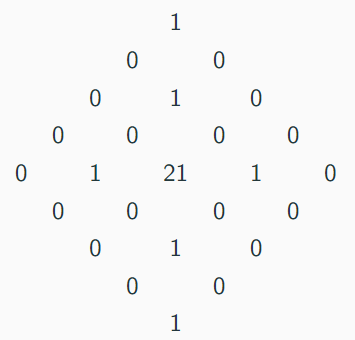
\includegraphics[width=0.9\textwidth]{CubicFourfoldHodgeDiamond.png} % first figure itself
        \caption*{Cubic fourfold}
    \end{minipage}\hfill
    \begin{minipage}{0.45\textwidth}
        \centering
        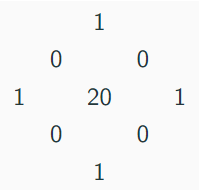
\includegraphics[width=0.4\textwidth]{K3diamond} % second figure itself
        \caption*{K3 surface}
    \end{minipage}
\end{figure}

\end{frame}

\begin{comment}
    \begin{frame}{The moduli space of cubic fourfolds}
    Both K3 surfaces and cubic threefolds have a Global Torelli theorem, meaning that a cubic fourfold is specified by the line $H^{3,1}\subset H^4$, the condition $H^{3,1}\perp h^2$ and furthermore $\eta\cup \eta =0, \eta \cup \overline{\eta}>0$ and so the period map lands in an open subset of a quadric in $\P^{21}$. Voisin proved that this is an open immersion.
\end{frame}
\end{comment}

\begin{frame}{Cubic fourfolds and K3 surfaces}
    If we take the primitive cohomology of the cubic fourfold, we get something that looks exactly like a K3 surface! However, the two have different signatures.
    To be able to compare them, we have to pass to a codimension one subspace. For the K3, we can always take the primitive cohomology. 
    
    \pause For \emph{special cubic fourfolds} we can find a class $T\in H^{2,2}(X,\mathbb{Z})$ and move to its orthogonal complement.
\end{frame}

\begin{frame}{Hasset's theorem}

    \begin{colorthm}{Hasset}{}
        The cubics containing an integral class $T$ as above form a family of irreducible divisors $\mathcal{C}_d$, nonempty iff (*) $d>6, d=0,2 \,( \mathrm{mod}\, 6)$. Moreover, the cubics in $\mathcal{C}_d$ have an associated K3 surface i.e. $\exists S$ such that $$H^2_{prim}(S)\simeq \langle h^2, T\rangle ^\perp$$
        precisely when (**) $d$ is not divisible by four, nine, or any odd prime $p =-1(\,\mathrm{ mod }\, 3)$
    \end{colorthm}
\end{frame}

\begin{frame}{Back to the rationality problem for cubic fourfolds}

    Implicit in Hasset's results is the conjecture that the special cubic fourfolds are rational. Intuitively, one has to blow up a surface in order to be birational to $\P^4$. Hence, we expect the rational cubic fourfolds to form a countable union of divisors, which is neither open nor closed, in stark contrast to the lower dimensional cases!
    
\end{frame}

\begin{frame}{The derived perspective}
    Kuznetsov presented a different viewpoint on the cubic fourfold using derived categories. The three line bundles $\mathcal{O}_X, \mathcal{O}_X(1), \mathcal{O}_X(2)$ form an exceptional collection and he defined the component $$\mathcal{A}_X=\langle \mathcal{O}_X, \mathcal{O}_X(1), \mathcal{O}_X(2)\rangle ^\perp\subset \mathcal{D}(X)$$\pause

    The HKR theorem guarantees that the Hochschild homology of $\mathcal{A}_X$ is the same as that of a K3 surface. \pause Kuznetsov showed that $\mathcal{A}_X$ is a \emph{Calabi-Yau 2} category and posed the conjecture:

    \begin{colorconj}{Kuznetsov}{}
        $X$ is rational if and only if there is a K3 surface $S$ such that $$\mathcal{D}(S)\simeq \mathcal{A}_X$$
    \end{colorconj}
    
\end{frame}


    
\begin{comment}
\begin{frame}{Why is the Kuznetsov component CY2?}
    
\end{frame}

\begin{frame}{Fundamental (Non)-example: cubics containing a plane}
    The case $d=8$ in Hassett's list obeys condition $*$ but not $**$. In fact, generically, $$\mathcal{A}_X\simeq \mathcal{D}(S,\alpha)$$is the derived category of a twisted K3 surface! When the Brauer class $\alpha \in H^2 (S, \mathcal{O}_S^\times)$ vanishes, the cubic fourfold $X$ is in the intersection $\mathcal{C}_8\cap \mathcal{C}_d$ for some $d$ in $**$, which is consistent with te rationality predictions.
\end{frame}

\end{comment}

\begin{frame}{Fundamental (non)-example: cubics containing a plane}
    The first nonempty item on Hasset's list consists of the cubics containing a plane. This is $\calC_8$ (the $8$ is comming from the intersection matrix $\begin{pmatrix}
        3 & 1 \\
        1 & 3
    \end{pmatrix}$). 
    \newline
    
    \pause This class of cubics is perhaps the most important one: Voisin used it to prove the Torelli theorem for cubic fourfolds, and Addington-Thomas showed that $\calC_8 \cap \calC_d \neq \emptyset$ for all other nonempty $\calC_d$ and used deformation theory out of $\calC_8$ to deduce that Hasset's and Kuznetsov's conjectures are in fact equivalent!
    
\end{frame}

\begin{frame}[fragile]{Cubics containing a plane: geometry}
    Projecting orthogonally out of a plane $P\subset \mathbb{P}^5$ gives a rational map 


        \[\begin{tikzcd}
            \P \mathcal{N}_{P/ \mathbb{P}^5} \simeq E \arrow[d] \arrow[r] & \mathrm{Bl}_P \mathbb{P}^5 \arrow[d, "\tau"] \arrow[rd, "\phi"] &      \\
            P \arrow[r]                             & \mathbb{P}^5 \arrow[r, dotted]                          & \mathbb{P}^2
        \end{tikzcd}\]

        In fact, $\mathrm{Bl}_P \P^5 = \P (\O(-1)\oplus \O^{\oplus 3})$. \pause The strict transform of $X$ is a quadric fibration $$\tilde{X}\rightarrow \P^2$$which geometrically can be thought of as follows: the $\P^2$ parametrizes 3-planes containing $P$, and $X$ intersects such a 3-plane in $P$ union a quadric. These quadrics are nonsingular outside the determinant locus, which is a sextic curve.
                      
\end{frame}

\begin{frame}{Cubics containing a plane: geometry}
Now, a generic quadric is isomorphic to $\P^1 \times \P^1$ and has exactly two rulings, parametrized by the connected components of the Fano variety of lines $$\scrF(\P^1 \times \P^1)=\P^1 \coprod \P^1$$
\pause A singular quadric is a cone, so has exactly one ruling: $$\tscrF(Q)=\P^1$$ \pause

If we define $S$ to be the space of rulings on the fibers, we see that it is a double cover of $\P^2$ branched along the sextic curve. Moreover, the relative Fano variety parametrizing lines in the fibers is a $\P^1$ bundle over this: $$\tscrF \xrightarrow{\pi_S} S \xrightarrow{\pi} \P^2$$
\pause In other words, for every $y\in \P^2$, the fiber of $\tscrF$ is equal to $\scrF(Q_y)$, the Fano variety of lines in the residual quadric corresponding to $y$.
\end{frame}

\begin{frame}{Twisted K3 surfaces}
    In fact, this $S$ is a K3 surface and $\tscrF \rightarrow S$ is a $\P^1$ bundle. \pause There is an obstruction cocycle $\alpha$ to this being a projectivization of a vector bundle, governed by the exact sequence $$1\rightarrow \mathbb{G}_m\rightarrow \mathrm{GL}\rightarrow \mathrm{PGL}\rightarrow 1$$ \pause

    We can consider \emph{twisted vector bundles} on $S$ which only satisfy the cocycle condition up to $\alpha$, and they have a derived category $\mathcal{D}(S,\alpha)$. 

    \begin{colorthm}{Bernardara's twisted projective bundle formula}{}
        There is a semiorthogonal decomposition $$\calD (\tscrF)=\langle \calD(S,\alpha), \calD(S)\rangle $$
    \end{colorthm}
\end{frame}

\begin{frame}[fragile]{Kuznetsov's equivalence}
    \begin{colorthm}{Kuznetsov}{}
        There is a derived equivalence $$\calA_X\simeq \calD(S,\alpha)$$
    \end{colorthm}
    \pause
    Idea: use FM kernel from the universal line $\tscrP\subset X \times \tscrF$ with ideal sheaf $\calI$ and its adjoint: 

      \[\begin{tikzcd}
        \calD(X) \arrow[r, "\Phi", bend left] & \calD(\tscrF) \arrow[l, "\Psi", bend left]            \\
        \calA_X \arrow[u, hook]               & {\calD(S,\alpha)} \arrow[u, hook] \arrow[l, "\simeq"]
        \end{tikzcd}\]

    
\end{frame}

\begin{frame}{Thanks!!}
    Thank you for your attention!
\end{frame}










    

\end{document}
